\documentclass[a4paper]{ctexart}
\usepackage[utf8]{inputenc}
\usepackage[a4paper]{geometry}
\usepackage{graphicx}
\usepackage{float}
\usepackage{hyperref}
\usepackage[heading = false]{ctex}
\usepackage{xcolor}
\usepackage{fontspec}
\usepackage{listings}
\usepackage{color}

\definecolor{dkgreen}{rgb}{0,0.6,0}
\definecolor{gray}{rgb}{0.5,0.5,0.5}
\definecolor{mauve}{rgb}{0.58,0,0.82}

\lstset{
  frame=tb,
  aboveskip=3mm,
  belowskip=3mm,
  showstringspaces=false,
  columns=flexible,
  basicstyle = \ttfamily,
  numbers=none,
  numberstyle=\tiny\color{gray},
  keywordstyle=\color{blue},
  commentstyle=\color{dkgreen},
  stringstyle=\color{mauve},
  breaklines=true,
  breakatwhitespace=true,
  tabsize=3
}
\pagestyle{plain}
\geometry{top=1.0cm, bottom=2.0cm}

\begin{document}
  \begin{titlepage}
      \songti
      \begin{center}
        \vspace*{2cm}
        
\includegraphics[width=0.7\textwidth]{../HDU.png}\\
        \vspace*{1cm}
        {\fontsize{36pt}{0}
          \textbf{机器学习实验\\报\quad 告\\}
        }
        \vspace*{12cm}
        {\fontsize{18pt}{0}
          \makebox[80pt]{\textbf{实验名称}} \underline{\makebox[250pt]{\Large 无监督学习之降维(NMF)}}\\
          \vspace*{0.5cm}
          \makebox[80pt]{\textbf{学\qquad 院}} \underline{\makebox[250pt]{\Large 通信工程学院}}\\
          \vspace*{0.5cm}
          \makebox[80pt]{\textbf{专\qquad 业}} \underline{\makebox[250pt]{\Large xxxx}}\\
          \vspace*{0.5cm}
          \makebox[80pt]{\textbf{学\qquad 号}} \underline{\makebox[250pt]{\Large xxxx}}\\
          \vspace*{0.5cm}
          \makebox[80pt]{\textbf{学生姓名}} \underline{\makebox[250pt]{\Large xxx}}\\
        }
      \end{center}
  \end{titlepage}

  \CTEXsetup[format={\Large\bfseries}]{section}

  \newpage
  \section{实验目的}
    \begin{enumerate}
      \item 理解无监督学习中NMF降维算法原理
      \item 掌握Sklearn实现基于NMF方法及应用
    \end{enumerate}

  \section{实验内容与要求}
    \begin{itemize}
      \item 使用算法:Kmeans
      \item 实现步骤
      \begin{enumerate}
        \item 建立工程并导入sklearn相关工具包
        \item 设置基本参数并加载数据
        \item 创建特征提取的对象NMF,使用PCA作为对比
        \item 降维后数据点的可视化
      \end{enumerate}
    \end{itemize}

  \section{实验程序与结果}
  \subsection{程序代码}
  \lstinputlisting[language=Python]{lab9.py}
  \subsection{运行结果}
  \begin{figure}[H]
    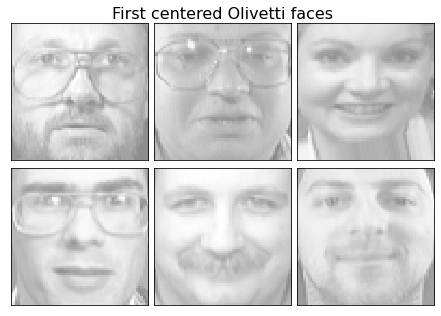
\includegraphics[width=1.0\textwidth]{fig/1.png}
  \end{figure}
  \newpage
  \begin{figure}[H]
    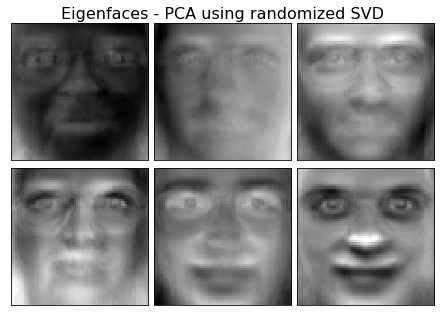
\includegraphics[width=1.0\textwidth]{fig/2.png}
    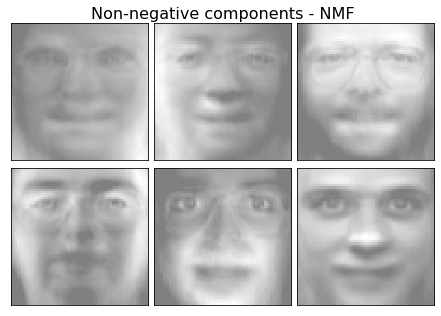
\includegraphics[width=1.0\textwidth]{fig/3.png}
  \end{figure}

  \section{实验问题解答与体会}
    本次实验使用了非负矩阵分解NMF方法对图像进行了降维和恢复,
    并且与基于随机SVD的PCA方法进行了对比,显示出NMF方法能够保留更多的信息

\end{document}
